\documentclass[10pt]{article}
\usepackage[utf8]{inputenc}
\usepackage[english]{babel}
\usepackage{mathrsfs}
\usepackage{graphicx}
\usepackage[euler]{textgreek}
\usepackage{fancyhdr} % For header
\usepackage{mdframed} % for boxes
\usepackage{geometry} % For margins
\usepackage{amsthm} % For theorems
\usepackage{amsmath,amsfonts} % For math


% For checklist
\usepackage{enumitem,amssymb}
\newlist{todolist}{itemize}{2}
\setlist[todolist]{label=$\square$}
\usepackage{pifont}
\newcommand{\cmark}{\ding{51}}%
\newcommand{\xmark}{\ding{55}}%
\newcommand{\done}{\rlap{$\square$}{\raisebox{2pt}{\large\hspace{1pt}\cmark}}%
\hspace{-2.5pt}}
\newcommand{\wontfix}{\rlap{$\square$}{\large\hspace{1pt}\xmark}}

 \geometry{
 a4paper,
 left=.75in,
 right=.75in,
 top=1in,
 }
 \newcommand{\bb}{\mathbb}
 \usepackage{sectsty}
\subsectionfont{\large\underline}
\fancyhf{}
\renewcommand\thesection{}
\renewcommand\thesubsection{}
\fancyhead[L]{\textbf{\leftmark\rightmark}}
\fancyhead[R]{\textbf{Spring 2020 PhD research}}

\rfoot{Page \thepage}
\pagestyle{fancy}

\theoremstyle{definition}
\newtheorem*{definition}{Definition}
\newtheorem*{example}{Example}
\newtheorem*{theorem}{Theorem}
\newtheorem*{lemma}{Lemma}
\newtheorem*{corollary}{Corrolary}
\setlength{\parskip}{1em}
\setlength{\parindent}{0pt}
\begin{document}


\section{Week 1}


\subsection{Data filtering}
Only use day 32.

Prevalence threshold. Only include taxa with more than 1 read in at least 30\% of samples.
This results in 39 taxa and 68 samples. The percent of the data is 46.3.

Then calculate absolute abundance.

The current covariate being used is


\subsection{Current code decisions}

\begin{itemize}
  \item $X$ is just the normal dataframe, so work needs to be done for each $\beta_j$. Should save on space and computation time.
  \item Currently beta loop has 1 iteration.
  \item Update is beta.new = beta.old - .1update
  \item V inv is phi A -1/2 r inv A -1/2
\end{itemize}



\subsection{Trying to locate code error}

\begin{itemize}
  \item Maybe revisit
  \item First loop: R inv
        Min.    1st Qu.     Median       Mean    3rd Qu.       Max.
  -0.5101610  0.0000000  0.0000000  0.0000554  0.0000000  1.7355810


  \item Getting an error first go: (in update beta function)

  \begin{verbatim}
      Error in h(simpleError(msg, call)) :
      error in evaluating the argument 'x' in selecting a method for function 'print': error in evaluating the argument 'physeq' in selecting a method for function 'taxa_names': object 'zebra2' not found
    In addition: Warning message:
    In paste0("beta ", rep(ASV_id, each = q), " = ", beta.new) :
      restarting interrupted promise evaluation Havent seen before
  \end{verbatim}

  FIXED. This was a problem with the ASV id argument having an old object.

\item
\begin{figure}[!htb]
	\centering
	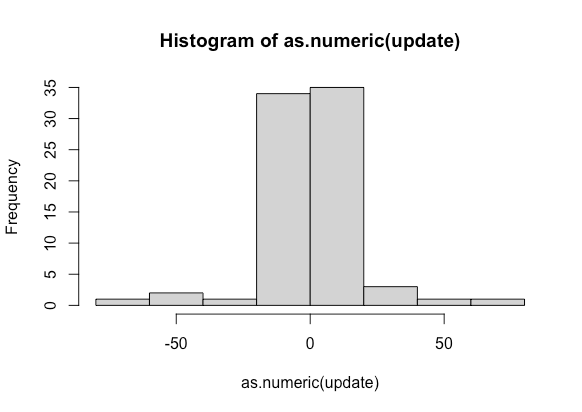
\includegraphics[width=0.45\textwidth]{img/Spring_2022_Journal-79240294.png}
	\caption{Histogram of update on first iteration }
	\label{}


\end{figure}
Check to make sure update items match the beta items they are subtracting? Yes.
\item

\begin{figure}[!htb]
	\centering
	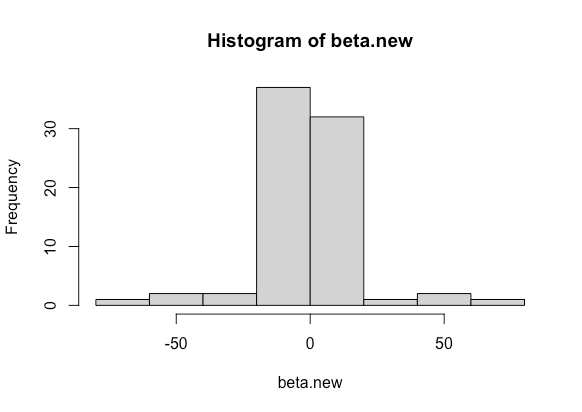
\includegraphics[width=0.45\textwidth]{img/Spring_2022_Journal-799ded17.png}
	\caption{Histogram of first betas }
	\label{}
\end{figure}

Check to make sure update items match the beta items they are subtracting? Yes.
\item \begin{figure}[!htb]
	\centering
	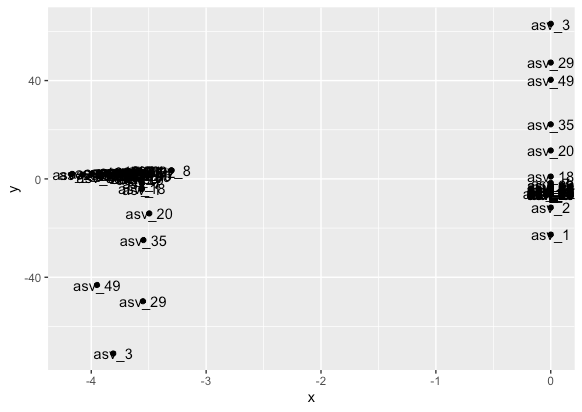
\includegraphics[width=0.45\textwidth]{img/Spring_2022_Journal-4c2e52e0.png}
	\caption{}
	\label{}
\end{figure}

\item Try with more iterations.
2nd iteration
\begin{figure}[!htb]
	\centering
	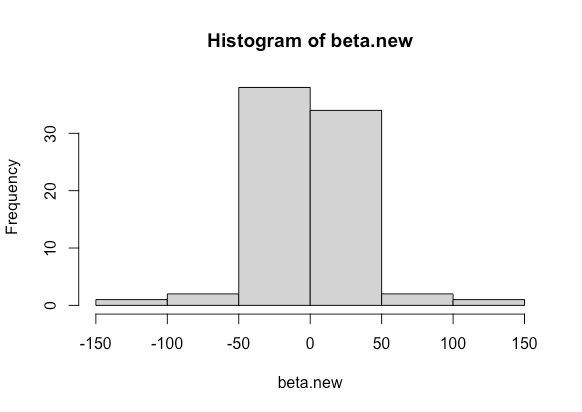
\includegraphics[width=0.45\textwidth]{img/Spring_2022_Journal-db626725.png}
	\caption{}
	\label{}
\end{figure}

\begin{figure}[!htb]
	\centering
	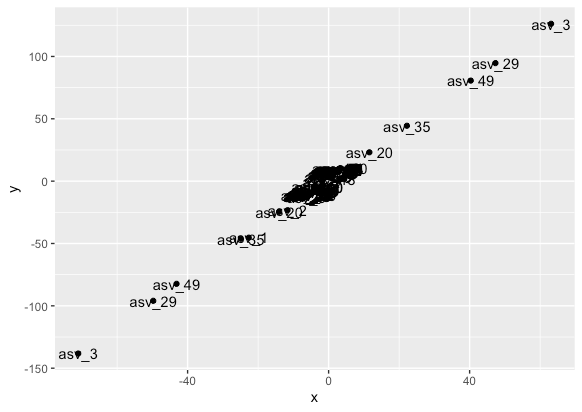
\includegraphics[width=0.45\textwidth]{img/Spring_2022_Journal-3fb47ab7.png}
	\caption{2nd iteration}
	\label{}
\end{figure}

\item Third iteration. Seems to be diverging.

\begin{figure}[!htb]
	\centering
	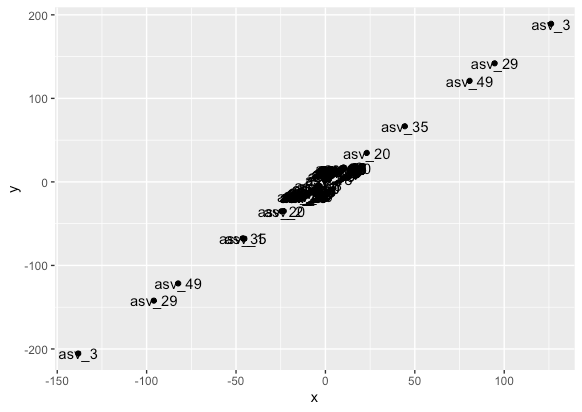
\includegraphics[width=0.45\textwidth]{img/Spring_2022_Journal-b7c8b87f.png}
	\caption{3rd iteration}
	\label{}
\end{figure}

It seems like the 'update' value isnt changing at all? Check this.

So one problem is that it doesn't change within loops. Does it change after calculating phi and rho? Check.

This is definetly some sort of problem.

Current value for update
\begin{verbatim}
   [1]  46.2016753 -47.3258792  -6.1901234  11.6566619  -4.7021419   3.6183032  -6.3952101
 [8]   6.3162696  -5.3106373   4.4185593  -6.6760288   5.7370180  -6.1907947   5.1419914
[15]  -6.6558117   5.5859662  -5.5437446   4.4394525  -6.7754318   5.6839888  21.3286876
[22] -22.2086941  -6.8085055   5.6762828  -5.1983832   4.4678220  -6.6312077   5.5477890
[29]  -3.3886343   2.5882506  -6.7459322   6.1195971  -4.4694171   3.4240657  -6.5218785
[36]   6.1263917  10.5371811 -11.5680454  -5.1779672   4.0250935  -6.2453704   5.1017399
[43]  -6.8097845   5.7015088  -6.1182510   4.9906303  -6.6345801   5.5203673  39.1947088
[50] -40.3184609   0.6062871  22.6626964  -3.7255341   2.6365179  -6.7033879   5.6927960
[57]  67.2184146 -63.0972211  -6.8193206   5.7064405  -4.9738631   3.8700908  -6.7519904
[64]   5.6536608  -4.7809281   3.7102062  -6.7036938   6.0152241   0.2275543  -0.9651037
[71]  -6.7608940   5.6802879  -5.8318696   4.7273785  -5.3378333   5.6281093  -1.7353577
[78]   1.6122465
\end{verbatim}


\item Now in Update phi r inv step

\begin{itemize}
  \item
	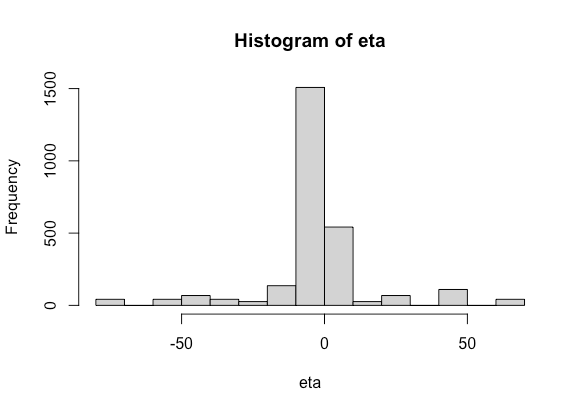
\includegraphics[width=0.45\textwidth]{img/Spring_2022_Journal-94ff41c0.png}


\item
\begin{verbatim}
  Browse[2]> summary(alpha)
     Min.   1st Qu.    Median      Mean   3rd Qu.      Max.
0.000e+00 0.000e+00 0.000e+00 7.977e+26 4.000e+00 5.037e+28
\end{verbatim}
\end{itemize}

This is already a huge problem, and looks to be from only one ASV.

(check if hessian and EEs are same? )

Again all the alphas are the same across samples. Why? Is this correct? Sort of. Since X is either 0 or 1.

\item Back to beta loop.

Seems like a bug was found> get\_eta step had beta, not beta.new. Try now.

Still think like I will need to recalculate A.

\begin{itemize}
  \item 2nd iteration


	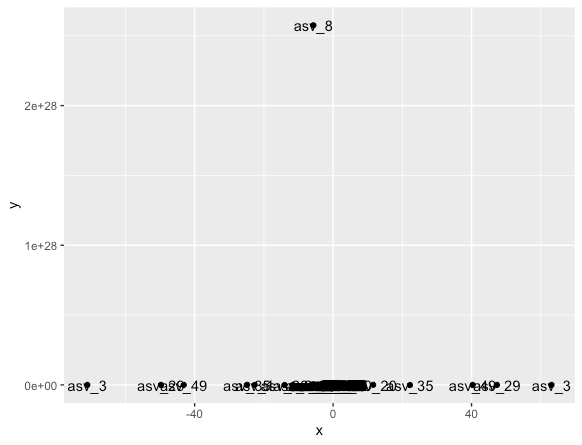
\includegraphics[width=0.45\textwidth]{img/Spring_2022_Journal-2025a7a8.png}



\item
	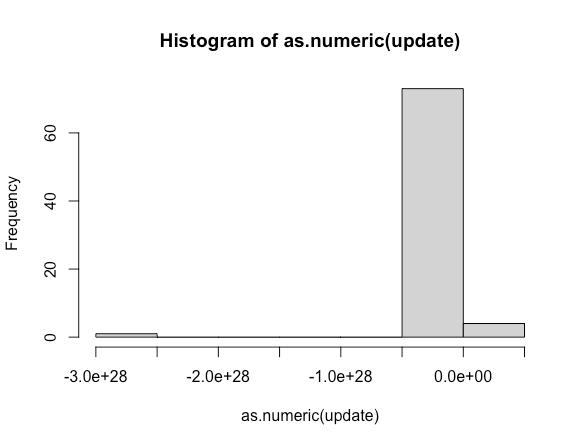
\includegraphics[width=0.45\textwidth]{img/Spring_2022_Journal-0491c15a.png}

\end{itemize}


\item On third loop, update is NaN. So is hessian. Probably because Vinv is now either 0 or NaN. Probably because of alpha. All partials are NaN.


What is the cause of this? Is this because phi is just 1? should we loop back?

Should do some checking about the partials.

Should test the

The gradient to find the direction towards zero of stepest decent which woudl be where zero would be? Confusion how this is the same as the estimating equations equaling zero.

And also that the sum is equal to zero, vs the matrix form.

Am i forgetting an X term??? in the hessian and GEE equations...
? No, this the X values are incorporated in the partials.
But are they in both the partials AND the GEE equations? No. So GEE is correct?

Is hessian a correct block matrix?




\item Now try constant times update. Trying beta.new = beta.old - .1 update

Somehow always gets a huge value? On like the second iteration. Range of beta values always goes up by a factor of 10 at least.

First run through:

\begin{verbatim}
Min. 1st Qu.  Median    Mean 3rd Qu.    Max.
0.01549 0.02411 0.02804 0.20715 0.03035 1.00000
\end{verbatim}

After only 1 beta iteration
\begin{verbatim}
  Min.   1st Qu.    Median      Mean   3rd Qu.      Max.
  0.00002   0.02163   0.03603   1.85100   0.10781 113.58914
\end{verbatim}

After 2:

\begin{verbatim}
       Min.   1st Qu.    Median      Mean   3rd Qu.      Max.
0.000e+00 0.000e+00 2.000e+01 1.439e+26 3.080e+03 9.087e+27
\end{verbatim}

\item test one more time if it should be +? No. even quicker huge. Actually is this correct? Geem code uses +. How is it different? Shoudl try again with loops.

\item Try going back and forth. At least one loop of going back to phi and rho estimating. With only one beta iteration.


\item R inv should change right? It does depend on rho and w, but it also depends on alpha. So it needs to change each iteration.

Also change R inv function to depend on alpha and alpha0 instead of X and beta.
Change R inv section of update phi R inv to call fxn.

But this shouldnt be the problems, since we still get the problem when the beta loops just once.

\item Try setting R -inv to be the identity matrix?

\item Check that hessian and estimating equations are correct and solve is doing what we think it is.

\item Code rearrranging. Move partials calculation to separate function. Update phi rho omega function no longer returns R inv since it is calculated in Beta step as needed depending on alpha values. DONE code runs. Still problem if multiple beta loops.

\item Things seem correct except one or two ASVs.


\item Going back to +. Try multiple beta loops (5) Then try (1) and back and forth with phi.

\item Look at residuals. At begining very right skewed. doing resid * phi results in larger numbers as phi starts off as > 1.

\item Trying on simulated dataset from orig paper. 45 percent prevalence.

Still problems. 2nd iteration already 10x9


\item Try going back and forth now. One beta iteration



\begin{verbatim}

[1] "Iteration: 1"
[1] "unstandardized residuals"
    Min.  1st Qu.   Median     Mean  3rd Qu.     Max.
-0.32868 -0.17361 -0.15113  0.07366 -0.03836 13.36048
[1] "phi = 0.939547462231508, omega  = 0.935468698041697 , rho = 3.17044241846978"
[1] "Beta iteration 1"
[1] "alpha"
   Min. 1st Qu.  Median    Mean 3rd Qu.    Max.
0.01549 0.02411 0.02804 0.20715 0.03035 1.00000
[1] "update"
    Min.  1st Qu.   Median     Mean  3rd Qu.     Max.
-61.9698  -6.3523   0.3406   0.0000   5.5856  66.1109
[1] "beta"
   Min. 1st Qu.  Median    Mean 3rd Qu.    Max.
-6.1970 -4.2508 -1.8167 -1.8396  0.5397  2.8024
Called from: update_beta(Y = Y, X = X, beta = beta, R_inv = R_inv, phi = phi,
    n_iter = 1, n = n, p = p, q = q, ASV_id, rho, omega, D = distance_matrix)
Browse[1]> Q
> # model!
> source(here::here("R","dm_cor_gee_clean.R"))
> zebra_res <- dm_cor_gee(Y = dat$Y, X = group, sample_id = dat$sampleID,
+                     ASV_id = taxa_names(zebrafish_ps), distance_matrix = D)
[1] "Iteration: 1"
[1] "unstandardized residuals"
    Min.  1st Qu.   Median     Mean  3rd Qu.     Max.
-0.32868 -0.17361 -0.15113  0.07366 -0.03836 13.36048
[1] "standardized residuals"
    Min.  1st Qu.   Median     Mean  3rd Qu.     Max.
-0.30881 -0.16312 -0.14199  0.06921 -0.03604 12.55280
[1] "phi = 0.939547462231508, omega  = 0.935468698041697 , rho = 3.17044241846978"
[1] "Beta iteration 1"
[1] "alpha"
   Min. 1st Qu.  Median    Mean 3rd Qu.    Max.
0.01549 0.02411 0.02804 0.20715 0.03035 1.00000
[1] "update"
    Min.  1st Qu.   Median     Mean  3rd Qu.     Max.
-61.9698  -6.3523   0.3406   0.0000   5.5856  66.1109
[1] "beta"
   Min. 1st Qu.  Median    Mean 3rd Qu.    Max.
-6.1970 -4.2508 -1.8167 -1.8396  0.5397  2.8024
Called from: update_beta(Y = Y, X = X, beta = beta, R_inv = R_inv, phi = phi,
    n_iter = 1, n = n, p = p, q = q, ASV_id, rho, omega, D = distance_matrix)
Browse[1]> c
[1] "Difference = 73.1214064026175"
[1] "Iteration: 2"
[1] "unstandardized residuals"
    Min.  1st Qu.   Median     Mean  3rd Qu.     Max.
 -9.8986  -0.0543  -0.0203   1.7148   0.1129 386.2322
[1] "standardized residuals"
      Min.    1st Qu.     Median       Mean    3rd Qu.       Max.
-0.0293348 -0.0001610 -0.0000601  0.0050819  0.0003345  1.1446128
[1] "phi = 0.00296353515610966, omega  = 0.983583744233043 , rho = 0.308232522541486"
[1] "Beta iteration 1"
[1] "alpha"
     Min.   1st Qu.    Median      Mean   3rd Qu.      Max.
 0.000024  0.015260  0.024415  0.833407  0.158479 25.868966
[1] "update"
    Min.  1st Qu.   Median     Mean  3rd Qu.     Max.
-19.0617  -2.4970  -1.3329   0.0000  -0.1486  55.5879
[1] "beta"
   Min. 1st Qu.  Median    Mean 3rd Qu.    Max.
-6.4988 -4.4549 -1.7234 -1.8396  0.3347  7.8160
Called from: update_beta(Y = Y, X = X, beta = beta, R_inv = R_inv, phi = phi,
    n_iter = 1, n = n, p = p, q = q, ASV_id, rho, omega, D = distance_matrix)
Browse[1]> c
[1] "Difference = 30.5331749772207"
[1] "Iteration: 3"
[1] "unstandardized residuals"
     Min.   1st Qu.    Median      Mean   3rd Qu.      Max.
 -24.2972   -0.0415   -0.0078    9.9096    0.2748 2818.1882
[1] "standardized residuals"
      Min.    1st Qu.     Median       Mean    3rd Qu.       Max.
-1.413e-03 -2.410e-06 -4.500e-07  5.762e-04  1.598e-05  1.639e-01
[1] "phi = 5.81411712568661e-05, omega  = 0.984549152947368 , rho = 0.614651231064176"
[1] "Beta iteration 1"
[1] "alpha"
     Min.   1st Qu.    Median      Mean   3rd Qu.      Max.
  0.00001   0.01081   0.01766   3.53512   0.32766 157.38310
[1] "update"
     Min.   1st Qu.    Median      Mean   3rd Qu.      Max.
-12.58427   0.01956   0.06204   0.00000   0.17577   7.83440
[1] "beta"
   Min. 1st Qu.  Median    Mean 3rd Qu.    Max.
-5.9998 -4.4254 -2.1959 -1.8396  0.3538  7.9364
Called from: update_beta(Y = Y, X = X, beta = beta, R_inv = R_inv, phi = phi,
    n_iter = 1, n = n, p = p, q = q, ASV_id, rho, omega, D = distance_matrix)
Browse[1]> c
[1] "Difference = 8.61011875874332"
[1] "Iteration: 4"
[1] "unstandardized residuals"
     Min.   1st Qu.    Median      Mean   3rd Qu.      Max.
 -23.9501   -0.0401   -0.0070    7.4950    0.2938 1796.3779
[1] "standardized residuals"
      Min.    1st Qu.     Median       Mean    3rd Qu.       Max.
-3.337e-03 -5.590e-06 -9.700e-07  1.044e-03  4.094e-05  2.503e-01
[1] "phi = 0.00013933155067034, omega  = 0.984796476225481 , rho = 0.440094621222131"
[1] "Beta iteration 1"
[1] "alpha"
     Min.   1st Qu.    Median      Mean   3rd Qu.      Max.
  0.00003   0.01035   0.01816   3.84221   0.32776 168.00334
[1] "update"
      Min.    1st Qu.     Median       Mean    3rd Qu.       Max.
-14.033385   0.004312   0.053323   0.000000   0.271548   7.106205
[1] "beta"
   Min. 1st Qu.  Median    Mean 3rd Qu.    Max.
-7.0599 -4.4007 -1.9964 -1.8396  0.3889  8.2196
Called from: update_beta(Y = Y, X = X, beta = beta, R_inv = R_inv, phi = phi,
    n_iter = 1, n = n, p = p, q = q, ASV_id, rho, omega, D = distance_matrix)
Browse[1]> c
[1] "Difference = 9.72467917960964"
[1] "Iteration: 5"
[1] "unstandardized residuals"
     Min.   1st Qu.    Median      Mean   3rd Qu.      Max.
 -24.1412   -0.0376   -0.0064    7.4793    0.3330 1292.1849
[1] "standardized residuals"
      Min.    1st Qu.     Median       Mean    3rd Qu.       Max.
-5.580e-03 -8.680e-06 -1.480e-06  1.729e-03  7.697e-05  2.987e-01
[1] "phi = 0.000231139860008589, omega  = 0.981520887502283 , rho = 0.369866079073633"
[1] "Beta iteration 1"
[1] "alpha"
     Min.   1st Qu.    Median      Mean   3rd Qu.      Max.
  0.00006   0.01129   0.01979   4.49665   0.29609 192.75334
[1] "update"
     Min.   1st Qu.    Median      Mean   3rd Qu.      Max.
-18.66292  -0.03128   0.04199   0.00000   0.41205  10.10912
[1] "beta"
   Min. 1st Qu.  Median    Mean 3rd Qu.    Max.
-8.3170 -4.3644 -2.1857 -1.8396  0.3966  8.6902
Called from: update_beta(Y = Y, X = X, beta = beta, R_inv = R_inv, phi = phi,
    n_iter = 1, n = n, p = p, q = q, ASV_id, rho, omega, D = distance_matrix)
Browse[1]> Q
> # model!
> source(here::here("R","dm_cor_gee_clean.R"))
> zebra_res <- dm_cor_gee(Y = dat$Y, X = group, sample_id = dat$sampleID,
+                     ASV_id = taxa_names(zebrafish_ps), distance_matrix = D)
[1] "Iteration: 1"
[1] "unstandardized residuals"
    Min.  1st Qu.   Median     Mean  3rd Qu.     Max.
-0.32868 -0.17361 -0.15113  0.07366 -0.03836 13.36048
[1] "standardized residuals"
    Min.  1st Qu.   Median     Mean  3rd Qu.     Max.
-0.30881 -0.16312 -0.14199  0.06921 -0.03604 12.55280
[1] "phi = 0.939547462231508, omega  = 0.935468698041697 , rho = 3.17044241846978"
[1] "Beta iteration 1"
[1] "alpha"
   Min. 1st Qu.  Median    Mean 3rd Qu.    Max.
0.01549 0.02411 0.02804 0.20715 0.03035 1.00000
[1] "update"
    Min.  1st Qu.   Median     Mean  3rd Qu.     Max.
-61.9698  -6.3523   0.3406   0.0000   5.5856  66.1109
[1] "beta"
   Min. 1st Qu.  Median    Mean 3rd Qu.    Max.
-6.1970 -4.2508 -1.8167 -1.8396  0.5397  2.8024
[1] "Difference = 73.1214064026175"
[1] "Iteration: 2"
[1] "unstandardized residuals"
    Min.  1st Qu.   Median     Mean  3rd Qu.     Max.
 -9.8986  -0.0543  -0.0203   1.7148   0.1129 386.2322
[1] "standardized residuals"
      Min.    1st Qu.     Median       Mean    3rd Qu.       Max.
-0.0293348 -0.0001610 -0.0000601  0.0050819  0.0003345  1.1446128
[1] "phi = 0.00296353515610966, omega  = 0.983583744233043 , rho = 0.308232522541486"
[1] "Beta iteration 1"
[1] "alpha"
     Min.   1st Qu.    Median      Mean   3rd Qu.      Max.
 0.000024  0.015260  0.024415  0.833407  0.158479 25.868966
[1] "update"
    Min.  1st Qu.   Median     Mean  3rd Qu.     Max.
-19.0617  -2.4970  -1.3329   0.0000  -0.1486  55.5879
[1] "beta"
   Min. 1st Qu.  Median    Mean 3rd Qu.    Max.
-6.4988 -4.4549 -1.7234 -1.8396  0.3347  7.8160
[1] "Difference = 30.5331749772207"
[1] "Iteration: 3"
[1] "unstandardized residuals"
     Min.   1st Qu.    Median      Mean   3rd Qu.      Max.
 -24.2972   -0.0415   -0.0078    9.9096    0.2748 2818.1882
[1] "standardized residuals"
      Min.    1st Qu.     Median       Mean    3rd Qu.       Max.
-1.413e-03 -2.410e-06 -4.500e-07  5.762e-04  1.598e-05  1.639e-01
[1] "phi = 5.81411712568661e-05, omega  = 0.984549152947368 , rho = 0.614651231064176"
[1] "Beta iteration 1"
[1] "alpha"
     Min.   1st Qu.    Median      Mean   3rd Qu.      Max.
  0.00001   0.01081   0.01766   3.53512   0.32766 157.38310
[1] "update"
     Min.   1st Qu.    Median      Mean   3rd Qu.      Max.
-12.58427   0.01956   0.06204   0.00000   0.17577   7.83440
[1] "beta"
   Min. 1st Qu.  Median    Mean 3rd Qu.    Max.
-5.9998 -4.4254 -2.1959 -1.8396  0.3538  7.9364
[1] "Difference = 8.61011875874332"
[1] "Iteration: 4"
[1] "unstandardized residuals"
     Min.   1st Qu.    Median      Mean   3rd Qu.      Max.
 -23.9501   -0.0401   -0.0070    7.4950    0.2938 1796.3779
[1] "standardized residuals"
      Min.    1st Qu.     Median       Mean    3rd Qu.       Max.
-3.337e-03 -5.590e-06 -9.700e-07  1.044e-03  4.094e-05  2.503e-01
[1] "phi = 0.00013933155067034, omega  = 0.984796476225481 , rho = 0.440094621222131"
[1] "Beta iteration 1"
[1] "alpha"
     Min.   1st Qu.    Median      Mean   3rd Qu.      Max.
  0.00003   0.01035   0.01816   3.84221   0.32776 168.00334
[1] "update"
      Min.    1st Qu.     Median       Mean    3rd Qu.       Max.
-14.033385   0.004312   0.053323   0.000000   0.271548   7.106205
[1] "beta"
   Min. 1st Qu.  Median    Mean 3rd Qu.    Max.
-7.0599 -4.4007 -1.9964 -1.8396  0.3889  8.2196
[1] "Difference = 9.72467917960964"
[1] "Iteration: 5"
[1] "unstandardized residuals"
     Min.   1st Qu.    Median      Mean   3rd Qu.      Max.
 -24.1412   -0.0376   -0.0064    7.4793    0.3330 1292.1849
[1] "standardized residuals"
      Min.    1st Qu.     Median       Mean    3rd Qu.       Max.
-5.580e-03 -8.680e-06 -1.480e-06  1.729e-03  7.697e-05  2.987e-01
[1] "phi = 0.000231139860008589, omega  = 0.981520887502283 , rho = 0.369866079073633"
[1] "Beta iteration 1"
[1] "alpha"
     Min.   1st Qu.    Median      Mean   3rd Qu.      Max.
  0.00006   0.01129   0.01979   4.49665   0.29609 192.75334
[1] "update"
     Min.   1st Qu.    Median      Mean   3rd Qu.      Max.
-18.66292  -0.03128   0.04199   0.00000   0.41205  10.10912
[1] "beta"
   Min. 1st Qu.  Median    Mean 3rd Qu.    Max.
-8.3170 -4.3644 -2.1857 -1.8396  0.3966  8.6902
[1] "Difference = 12.9032787639054"
[1] "Iteration: 6"
[1] "unstandardized residuals"
     Min.   1st Qu.    Median      Mean   3rd Qu.      Max.
 -24.3482   -0.0361   -0.0057   11.0754    0.3874 1013.8554
[1] "standardized residuals"
      Min.    1st Qu.     Median       Mean    3rd Qu.       Max.
-3.938e-03 -5.840e-06 -9.200e-07  1.791e-03  6.266e-05  1.640e-01
[1] "phi = 0.000161748619031987, omega  = 0.977301954235005 , rho = 0.426519229141335"
[1] "Beta iteration 1"
[1] "alpha"
     Min.   1st Qu.    Median      Mean   3rd Qu.      Max.
  0.00011   0.01054   0.02011   5.82520   0.35510 239.40531
[1] "update"
     Min.   1st Qu.    Median      Mean   3rd Qu.      Max.
-23.72076  -0.03532   0.06225   0.00000   0.88363  12.20260
[1] "beta"
    Min.  1st Qu.   Median     Mean  3rd Qu.     Max.
-10.0963  -4.2798  -2.0745  -1.8396   0.3993   9.0211
[1] "Difference = 17.0379943115704"
[1] "Iteration: 7"
[1] "unstandardized residuals"
     Min.   1st Qu.    Median      Mean   3rd Qu.      Max.
 -24.0014   -0.0324   -0.0046   24.7836    0.4011 2630.8079
[1] "standardized residuals"
      Min.    1st Qu.     Median       Mean    3rd Qu.       Max.
-6.732e-04 -9.100e-07 -1.300e-07  6.952e-04  1.125e-05  7.379e-02
[1] "phi = 2.80500340906498e-05, omega  = 0.979940749278977 , rho = 0.767286381667904"
[1] "Beta iteration 1"
[1] "alpha"
     Min.   1st Qu.    Median      Mean   3rd Qu.      Max.
  0.00001   0.01153   0.02309   7.19580   0.36725 277.28483
[1] "update"
      Min.    1st Qu.     Median       Mean    3rd Qu.       Max.
-20.567520   0.006673   0.049880   0.000000   0.864810  18.328470
[1] "beta"
    Min.  1st Qu.   Median     Mean  3rd Qu.     Max.
-12.0073  -4.2858  -1.5401  -1.8396   0.4062   9.0784
[1] "Difference = 15.8878677458046"
[1] "Iteration: 8"
[1] "unstandardized residuals"
    Min.  1st Qu.   Median     Mean  3rd Qu.     Max.
 -22.289   -0.035   -0.005   60.270    0.406 6753.782
[1] "standardized residuals"
      Min.    1st Qu.     Median       Mean    3rd Qu.       Max.
-9.624e-05 -1.490e-07 -2.000e-08  2.602e-04  1.753e-06  2.916e-02
[1] "phi = 4.31785512143427e-06, omega  = 0.981709982661524 , rho = 0.961916134714736"
[1] "Beta iteration 1"
[1] "alpha"
     Min.   1st Qu.    Median      Mean   3rd Qu.      Max.
  0.00000   0.01248   0.02315   8.25611   0.51991 286.74174
[1] "update"
      Min.    1st Qu.     Median       Mean    3rd Qu.       Max.
-14.016899   0.004457   0.025964   0.000000   0.518477  14.558641
[1] "beta"
    Min.  1st Qu.   Median     Mean  3rd Qu.     Max.
-13.3450  -4.2257  -1.0646  -1.8396   0.4119   9.0873
[1] "Difference = 9.80437753991997"
[1] "Iteration: 9"
[1] "unstandardized residuals"
     Min.   1st Qu.    Median      Mean   3rd Qu.      Max.
  -19.672    -0.030    -0.005   101.003     0.438 11249.150
[1] "standardized residuals"
      Min.    1st Qu.     Median       Mean    3rd Qu.       Max.
-3.053e-05 -4.700e-08 -7.000e-09  1.568e-04  6.800e-07  1.746e-02
[1] "phi = 1.55207729785946e-06, omega  = 0.983803047522562 , rho = 0.868270247649568"
[1] "Beta iteration 1"
[1] "alpha"
     Min.   1st Qu.    Median      Mean   3rd Qu.      Max.
  0.00000   0.01256   0.02430   9.55604   0.65224 289.15841
[1] "update"
     Min.   1st Qu.    Median      Mean   3rd Qu.      Max.
-15.37337   0.00853   0.03123   0.00000   0.46301  11.10487
[1] "beta"
    Min.  1st Qu.   Median     Mean  3rd Qu.     Max.
-14.8315  -4.1920  -1.0642  -1.8396   0.4288   9.0904
[1] "Difference = 7.98261948839764"
[1] "Iteration: 10"
[1] "unstandardized residuals"
     Min.   1st Qu.    Median      Mean   3rd Qu.      Max.
  -18.309    -0.029    -0.004   129.332     0.434 13959.282
[1] "standardized residuals"
      Min.    1st Qu.     Median       Mean    3rd Qu.       Max.
-1.833e-05 -2.900e-08 -4.000e-09  1.295e-04  4.340e-07  1.397e-02
[1] "phi = 1.00102793904902e-06, omega  = 0.983523869706203 , rho = 0.773146920273194"
[1] "Beta iteration 1"
[1] "alpha"
    Min.  1st Qu.   Median     Mean  3rd Qu.     Max.
  0.0000   0.0136   0.0256  10.5181   1.0068 291.3046
[1] "update"
     Min.   1st Qu.    Median      Mean   3rd Qu.      Max.
-18.19715   0.01472   0.03910   0.00000   0.50783   7.87463
[1] "beta"
    Min.  1st Qu.   Median     Mean  3rd Qu.     Max.
-16.6097  -4.1478  -1.0636  -1.8396   0.4337   9.0925
[1] "Difference = 7.70284144296252"
[1] "Iteration: 11"
[1] "unstandardized residuals"
     Min.   1st Qu.    Median      Mean   3rd Qu.      Max.
  -17.543    -0.031    -0.004   138.071     0.431 13422.175
[1] "standardized residuals"
      Min.    1st Qu.     Median       Mean    3rd Qu.       Max.
-1.812e-05 -3.200e-08 -4.000e-09  1.426e-04  4.450e-07  1.386e-02
[1] "phi = 1.032894614361e-06, omega  = 0.97736747447489 , rho = 0.74371714175976"
[1] "Beta iteration 1"
[1] "alpha"
     Min.   1st Qu.    Median      Mean   3rd Qu.      Max.
  0.00000   0.01464   0.02724  11.27012   1.10443 293.65488
[1] "update"
     Min.   1st Qu.    Median      Mean   3rd Qu.      Max.
-20.73626   0.01951   0.04600   0.00000   0.58505   4.40622
[1] "beta"
    Min.  1st Qu.   Median     Mean  3rd Qu.     Max.
-18.6416  -4.1024  -1.0627  -1.8396   0.4474   9.0946
[1] "Difference = 9.52078537828392"
[1] "Iteration: 12"
[1] "unstandardized residuals"
     Min.   1st Qu.    Median      Mean   3rd Qu.      Max.
  -17.379    -0.036    -0.004   155.679     0.433 19057.502
[1] "standardized residuals"
      Min.    1st Qu.     Median       Mean    3rd Qu.       Max.
-1.720e-05 -3.600e-08 -4.000e-09  1.541e-04  4.280e-07  1.886e-02
[1] "phi = 9.8959962990127e-07, omega  = 0.942937105631337 , rho = 1.16337548753744"
[1] "Beta iteration 1"
[1] "alpha"
     Min.   1st Qu.    Median      Mean   3rd Qu.      Max.
  0.00000   0.01520   0.02992  11.77454   1.11314 296.63069
[1] "update"
      Min.    1st Qu.     Median       Mean    3rd Qu.       Max.
-18.936152   0.003131   0.038862   0.000000   0.499806   4.293101
[1] "beta"
    Min.  1st Qu.   Median     Mean  3rd Qu.     Max.
-20.4962  -4.0756  -1.0616  -1.8396   0.4721   9.0966
[1] "Difference = 9.14039783751598"
[1] "Iteration: 13"
[1] "unstandardized residuals"
    Min.  1st Qu.   Median     Mean  3rd Qu.     Max.
  -15.77    -0.03     0.00   245.13     0.46 51778.12
[1] "standardized residuals"
      Min.    1st Qu.     Median       Mean    3rd Qu.       Max.
-4.615e-06 -1.000e-08 -1.000e-09  7.172e-05  1.350e-07  1.515e-02
[1] "phi = 2.92597293152538e-07, omega  = 0.87531027288368 , rho = 2.48890365167915"
[1] "Beta iteration 1"
[1] "alpha"
     Min.   1st Qu.    Median      Mean   3rd Qu.      Max.
  0.00000   0.01679   0.03344  13.39275   1.12181 298.59983
[1] "update"
     Min.   1st Qu.    Median      Mean   3rd Qu.      Max.
-6.136997 -0.003978  0.008558  0.000000  0.149141  4.202295
[1] "beta"
    Min.  1st Qu.   Median     Mean  3rd Qu.     Max.
-21.0967  -4.0554  -1.0611  -1.8396   0.4762   9.0972
[1] "Difference = 3.67821574427527"
[1] "Iteration: 14"
[1] "unstandardized residuals"
    Min.  1st Qu.   Median     Mean  3rd Qu.     Max.
  -15.62    -0.03     0.00   294.70     0.47 72050.71
[1] "standardized residuals"
      Min.    1st Qu.     Median       Mean    3rd Qu.       Max.
-2.590e-06 -6.000e-09  0.000e+00  4.886e-05  7.800e-08  1.195e-02
[1] "phi = 1.65792585919558e-07, omega  = 0.839776237723401 , rho = 3.4180370064409"
[1] "Beta iteration 1"
[1] "alpha"
     Min.   1st Qu.    Median      Mean   3rd Qu.      Max.
  0.00000   0.01796   0.03444  14.00361   1.12401 298.63102
[1] "update"
     Min.   1st Qu.    Median      Mean   3rd Qu.      Max.
-2.977099 -0.003386  0.003406  0.000000  0.064081  2.237480
[1] "beta"
    Min.  1st Qu.   Median     Mean  3rd Qu.     Max.
-21.3456  -4.0503  -1.0609  -1.8396   0.4774   9.0976
[1] "Difference = 1.799666661543"
[1] "Iteration: 15"
[1] "unstandardized residuals"
    Min.  1st Qu.   Median     Mean  3rd Qu.     Max.
  -15.91    -0.03     0.00   321.93     0.47 82856.93
[1] "standardized residuals"
      Min.    1st Qu.     Median       Mean    3rd Qu.       Max.
-2.040e-06 -4.000e-09  0.000e+00  4.129e-05  6.100e-08  1.063e-02
[1] "phi = 1.28248839357702e-07, omega  = 0.828273602668781 , rho = 3.7252933030863"
[1] "Beta iteration 1"
[1] "alpha"
     Min.   1st Qu.    Median      Mean   3rd Qu.      Max.
  0.00000   0.01818   0.03485  14.29110   1.12504 298.59553
[1] "update"
     Min.   1st Qu.    Median      Mean   3rd Qu.      Max.
-2.350114 -0.002299  0.002545  0.000000  0.044816  1.784247
[1] "beta"
    Min.  1st Qu.   Median     Mean  3rd Qu.     Max.
-21.5192  -4.0463  -1.0608  -1.8396   0.4782   9.0978
[1] "Difference = 1.36297655529556"
[1] "Iteration: 16"
[1] "unstandardized residuals"
    Min.  1st Qu.   Median     Mean  3rd Qu.     Max.
  -16.13    -0.03     0.00   343.41     0.48 91301.89
[1] "standardized residuals"
      Min.    1st Qu.     Median       Mean    3rd Qu.       Max.
-1.724e-06 -4.000e-09  0.000e+00  3.671e-05  5.100e-08  9.760e-03
[1] "phi = 1.06895154366371e-07, omega  = 0.821954985685942 , rho = 3.89260965287554"
[1] "Beta iteration 1"
[1] "alpha"
     Min.   1st Qu.    Median      Mean   3rd Qu.      Max.
  0.00000   0.01834   0.03513  14.46801   1.12580 298.57293
[1] "update"
     Min.   1st Qu.    Median      Mean   3rd Qu.      Max.
-2.009067 -0.001680  0.002094  0.000000  0.034465  1.545656
[1] "beta"
    Min.  1st Qu.   Median     Mean  3rd Qu.     Max.
-21.6570  -4.0429  -1.0606  -1.8396   0.4788   9.0981
[1] "Difference = 1.14164129574494"
[1] "Iteration: 17"
[1] "unstandardized residuals"
    Min.  1st Qu.   Median     Mean  3rd Qu.     Max.
  -16.33    -0.03     0.00   362.13     0.48 98572.87
[1] "standardized residuals"
      Min.    1st Qu.     Median       Mean    3rd Qu.       Max.
-1.509e-06 -3.000e-09  0.000e+00  3.346e-05  4.400e-08  9.109e-03
[1] "phi = 9.24101535408146e-08, omega  = 0.817752143524932 , rho = 4.001984252125"
[1] "Beta iteration 1"
[1] "alpha"
     Min.   1st Qu.    Median      Mean   3rd Qu.      Max.
  0.00000   0.01848   0.03537  14.59056   1.12642 298.55984
[1] "update"
     Min.   1st Qu.    Median      Mean   3rd Qu.      Max.
-1.783508 -0.001677  0.001754  0.000000  0.029174  1.387214
[1] "beta"
    Min.  1st Qu.   Median     Mean  3rd Qu.     Max.
-21.7730  -4.0400  -1.0605  -1.8396   0.4793   9.0982
[1] "Difference = 1.00252084244208"
[1] "Iteration: 18"
[1] "unstandardized residuals"
     Min.   1st Qu.    Median      Mean   3rd Qu.      Max.
   -16.50     -0.03      0.00    379.18      0.48 105113.72
[1] "standardized residuals"
      Min.    1st Qu.     Median       Mean    3rd Qu.       Max.
-1.348e-06 -3.000e-09  0.000e+00  3.098e-05  4.000e-08  8.588e-03
[1] "phi = 8.17024565180398e-08, omega  = 0.81512168259833 , rho = 4.07040272560558"
[1] "Beta iteration 1"
[1] "alpha"
     Min.   1st Qu.    Median      Mean   3rd Qu.      Max.
  0.00000   0.01860   0.03557  14.68128   1.12696 298.55321
[1] "update"
     Min.   1st Qu.    Median      Mean   3rd Qu.      Max.
-1.624484 -0.001357  0.001587  0.000000  0.025886  1.275652
[1] "beta"
   Min. 1st Qu.  Median    Mean 3rd Qu.    Max.
-21.875  -4.037  -1.060  -1.840   0.480   9.098
[1] "Difference = 0.909333461307958"
[1] "Iteration: 19"
[1] "unstandardized residuals"
     Min.   1st Qu.    Median      Mean   3rd Qu.      Max.
   -16.67     -0.03      0.00    395.15      0.49 111172.40
[1] "standardized residuals"
      Min.    1st Qu.     Median       Mean    3rd Qu.       Max.
-1.222e-06 -2.000e-09  0.000e+00  2.898e-05  3.600e-08  8.152e-03
[1] "phi = 7.33305412394345e-08, omega  = 0.81275529367871 , rho = 4.13181563693982"
[1] "Beta iteration 1"
[1] "alpha"
     Min.   1st Qu.    Median      Mean   3rd Qu.      Max.
  0.00000   0.01871   0.03574  14.75118   1.12743 298.55116
[1] "update"
     Min.   1st Qu.    Median      Mean   3rd Qu.      Max.
-1.496403 -0.001123  0.001456  0.000000  0.023598  1.182527
[1] "beta"
    Min.  1st Qu.   Median     Mean  3rd Qu.     Max.
-21.9653  -4.0348  -1.0603  -1.8396   0.4807   9.0986
[1] "Difference = 0.834171847811243"
[1] "Iteration: 20"
[1] "unstandardized residuals"
     Min.   1st Qu.    Median      Mean   3rd Qu.      Max.
   -16.82     -0.03      0.00    410.29      0.49 116852.54
[1] "standardized residuals"
      Min.    1st Qu.     Median       Mean    3rd Qu.       Max.
-1.120e-06 -2.000e-09  0.000e+00  2.732e-05  3.300e-08  7.780e-03
[1] "phi = 6.65784120493533e-08, omega  = 0.81109333216788 , rho = 4.17480938728343"
[1] "Beta iteration 1"
[1] "alpha"
     Min.   1st Qu.    Median      Mean   3rd Qu.      Max.
  0.00000   0.01882   0.03671  14.80723   1.12785 298.55240
[1] "update"
      Min.    1st Qu.     Median       Mean    3rd Qu.       Max.
-1.3961088 -0.0009499  0.0013521  0.0000000  0.0218359  1.1091146
[1] "beta"
    Min.  1st Qu.   Median     Mean  3rd Qu.     Max.
-22.0476  -4.0324  -1.0603  -1.8396   0.4813   9.0987
[1] "Difference = 0.775798299095333"
[1] "Iteration: 21"
[1] "unstandardized residuals"
     Min.   1st Qu.    Median      Mean   3rd Qu.      Max.
   -16.96     -0.03      0.00    424.84      0.49 122251.16
[1] "standardized residuals"
      Min.    1st Qu.     Median       Mean    3rd Qu.       Max.
-1.034e-06 -2.000e-09  0.000e+00  2.591e-05  3.000e-08  7.454e-03
[1] "phi = 6.09768859792844e-08, omega  = 0.809388414671349 , rho = 4.21959678375907"
[1] "Beta iteration 1"
[1] "alpha"
     Min.   1st Qu.    Median      Mean   3rd Qu.      Max.
  0.00000   0.01891   0.03676  14.85325   1.12823 298.55606
[1] "update"
      Min.    1st Qu.     Median       Mean    3rd Qu.       Max.
-1.3088934 -0.0008111  0.0011964  0.0000000  0.0203318  1.0435144
[1] "beta"
    Min.  1st Qu.   Median     Mean  3rd Qu.     Max.
-22.1231  -4.0303  -1.0602  -1.8396   0.4818   9.0988
[1] "Difference = 0.724929256292401"
[1] "Iteration: 22"
[1] "unstandardized residuals"
     Min.   1st Qu.    Median      Mean   3rd Qu.      Max.
   -17.10     -0.03      0.00    438.86      0.49 127406.42
[1] "standardized residuals"
      Min.    1st Qu.     Median       Mean    3rd Qu.       Max.
-9.620e-07 -2.000e-09  0.000e+00  2.469e-05  2.700e-08  7.167e-03
[1] "phi = 5.6253998469363e-08, omega  = 0.808112293735121 , rho = 4.2508573317048"
[1] "Beta iteration 1"
[1] "alpha"
     Min.   1st Qu.    Median      Mean   3rd Qu.      Max.
  0.00000   0.01900   0.03677  14.89208   1.12858 298.56155
[1] "update"
      Min.    1st Qu.     Median       Mean    3rd Qu.       Max.
-1.2376627 -0.0007025  0.0010839  0.0000000  0.0191143  0.9896530
[1] "beta"
    Min.  1st Qu.   Median     Mean  3rd Qu.     Max.
-22.1930  -4.0282  -1.0601  -1.8396   0.4823   9.0989
[1] "Difference = 0.683596353407489"
[1] "Iteration: 23"
[1] "unstandardized residuals"
     Min.   1st Qu.    Median      Mean   3rd Qu.      Max.
   -17.22     -0.03      0.00    452.49      0.49 132372.85
[1] "standardized residuals"
      Min.    1st Qu.     Median       Mean    3rd Qu.       Max.
-8.990e-07 -2.000e-09  0.000e+00  2.362e-05  2.500e-08  6.910e-03
[1] "phi = 5.21985800496743e-08, omega  = 0.807087454024426 , rho = 4.27629557449581"
[1] "Beta iteration 1"
[1] "alpha"
     Min.   1st Qu.    Median      Mean   3rd Qu.      Max.
  0.00000   0.01909   0.03677  14.92542   1.12890 298.56839
[1] "update"
      Min.    1st Qu.     Median       Mean    3rd Qu.       Max.
-1.1767636 -0.0006142  0.0010144  0.0000000  0.0180836  0.9431323
[1] "beta"
    Min.  1st Qu.   Median     Mean  3rd Qu.     Max.
-22.2583  -4.0263  -1.0600  -1.8396   0.4828   9.0990
[1] "Difference = 0.648328105483543"
[1] "Iteration: 24"
[1] "unstandardized residuals"
     Min.   1st Qu.    Median      Mean   3rd Qu.      Max.
   -17.35     -0.03      0.00    465.79      0.49 137182.89
[1] "standardized residuals"
      Min.    1st Qu.     Median       Mean    3rd Qu.       Max.
-8.440e-07 -2.000e-09  0.000e+00  2.267e-05  2.400e-08  6.677e-03
[1] "phi = 4.86706590722903e-08, omega  = 0.806196366262477 , rho = 4.29792968866025"
[1] "Beta iteration 1"
[1] "alpha"
     Min.   1st Qu.    Median      Mean   3rd Qu.      Max.
  0.00000   0.01909   0.03678  14.95445   1.12921 298.57626
[1] "update"
      Min.    1st Qu.     Median       Mean    3rd Qu.       Max.
-1.1235722 -0.0005412  0.0009542  0.0000000  0.0171907  0.9020291
[1] "beta"
    Min.  1st Qu.   Median     Mean  3rd Qu.     Max.
-22.3197  -4.0244  -1.0600  -1.8396   0.4832   9.0991
[1] "Difference = 0.617539235770946"
[1] "Iteration: 25"
[1] "unstandardized residuals"
     Min.   1st Qu.    Median      Mean   3rd Qu.      Max.
   -17.46     -0.03      0.00    478.83      0.49 141859.99
[1] "standardized residuals"
      Min.    1st Qu.     Median       Mean    3rd Qu.       Max.
-7.960e-07 -2.000e-09  0.000e+00  2.182e-05  2.200e-08  6.464e-03
[1] "phi = 4.55692681244084e-08, omega  = 0.80541706862667 , rho = 4.31647868718837"
[1] "Beta iteration 1"
[1] "alpha"
     Min.   1st Qu.    Median      Mean   3rd Qu.      Max.
  0.00000   0.01909   0.03678  14.98010   1.12949 298.58490
[1] "update"
      Min.    1st Qu.     Median       Mean    3rd Qu.       Max.
-1.0765919 -0.0004804  0.0009014  0.0000000  0.0164077  0.8653577
[1] "beta"
    Min.  1st Qu.   Median     Mean  3rd Qu.     Max.
-22.3777  -4.0226  -1.0599  -1.8396   0.4836   9.0992
[1] "Difference = 0.590359570128033"

\end{verbatim}



\item It looks like it is working? With +, and only 1 update each. And a small update.

\item Wondering if a separate checklist and journal file would be a good idea.


\item I THINK IT IS RUNNING!

Things i did:

\begin{itemize}
  \item Change from - to +
  \item First do phi/rho/omega loop, then ONE beta loop. With update of .1 scaled.
  \item About a 2.5 min runtime with convergence defined as sum of absolute difference between beta values < .1. 225 iterations
  \item
\end{itemize}

\item Try removing step update.

\begin{itemize}
  \item \begin{verbatim}
    [1] "Iteration: 1"
  [1] "phi = 0.939547462231508, omega  = 0.935468698041697 , rho = 3.17044241846978"
  [1] "Beta iteration 1"
  [1] "Difference = 731.214064026175"
  [1] "Iteration: 2"
  [1] "phi = 1.74415189832243e-55, omega  = 0 , rho = 363.857722495099"
  [1] "Beta iteration 1"
  [1] "Difference = 0"
  \end{verbatim}

  \item Try .5 Still only 2 loops.
\end{itemize}

\item Graphs:


\item \textbf{Meeting}
\item Check eigeenvalues of update and scalar by minimum.

\item Implement line search.
Numerical Optimization book ch 11.2

\end{itemize}


\section{Week 2}

Next steps (from paper)
\begin{enumerate}
  \item Currently 39 taxa across 48 samples, Increase number of taxa, increase percent zero
  \item Try increasing covariates
  \item Think about genus level analysis
  \item Choose $\alpha$ more automatically (simple line search)
  \item How to test significance of $\beta$? Role of $\omega$ in this test.
  \item Simulation
\end{enumerate}
Start working on presentation, which should motivate and give a good todo on the way. Going over definitions of working correlation matrix, GEE equations, and update rho and beta steps. Then will include questions (3) and (5). Include line search if implemented. Data analysis results? TBD.

Goal implement the line search: (write up)

Work on presenting the data analysis portion on the presentation.

Today's agenda and order:
\begin{itemize}
  \item Re-do analysis: number 1 and 2: Increase number of taxa.(done) Increase covariates.
  \item Probably not writing this up yet, wait for line search step. But can include the data preprocessing slide
  \item Implement and write up line search
  \item Compare results for independence, different algorithm
  \item Calculate sandwhich estimator, idenetify significance, figure out which ASVs corresponding to.
\end{itemize}


\subsection{Meeting agenda:}
Creating presentation: Did we forget that the phylogenetic portion has to be positive?

Ask about how to make presentations longer, always rushed and quick. Ask for feedback.

If I use minus hessian and minus it stalls out on 2nd iteration. Weird that this doesnt work?

What should the initial value of rho and omega be in the nls optim? Currently always .5 and 1. Would this change results?

\subsection{ Item 1 Increase number of taxa}
Procesing and filtering, and covariate information:


Still had to match tip labels. Using phyloseq object from Tom (in paired_data_ and ps Box folder) and tree from?

Only looking at day 32
Unfiltered day 32 has 3895 taxa across 68 samples. 98.4 percent zero entries

Keep ASV if present in at least 10 \% of samples

Results in 166 taxa in 68 samples. 75\% of data are zero.

Covariates. 1 if NC, 0 if ND.

RESULTS:

\begin{verbatim}
  [1] "Iteration: 149"
[1] "phi = 7.98731653686342e-12, omega  = 0.997838301680261 , rho = 0.104950295482753"
[1] "Beta iteration 1"
[1] "Difference = 0.0998224219301233"
\end{verbatim}

So not great, and very different from previous.
So high an omega would mean all weight is towards the compositional correlation. So low an rho means.

Also had a slower run time. 20 minutes.

Some interesting plots! Seems like something happens around iteration 60 that completely changes the results.

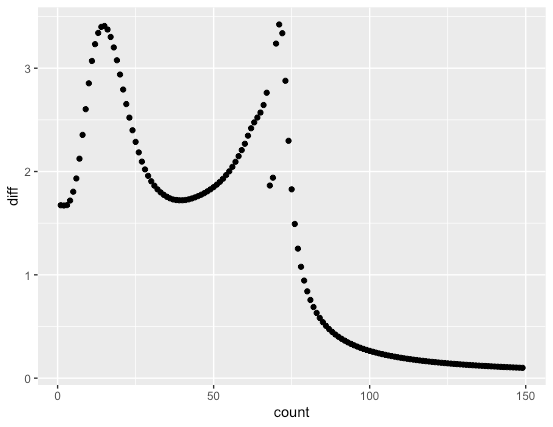
\includegraphics[width=0.35\textwidth]{img/Spring_2022_Journal-c6b97817.png}

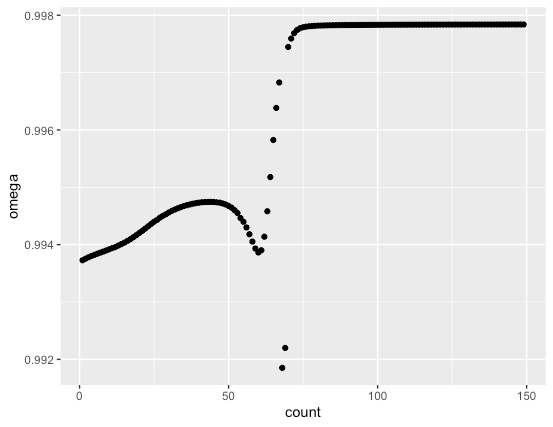
\includegraphics[width=0.95\textwidth]{img/Spring_2022_Journal-8a414f07.png}


\subsection{Initial values of rho and omega in nlsoptim}

Should we use .5 and 1 or the previous iteration values?

What would happen if we used .5 and 10?

Seems like it makes it very unstable.

Stability seems to not be great. Might be finding local mins?

(Note, changing max iterations to 50)

	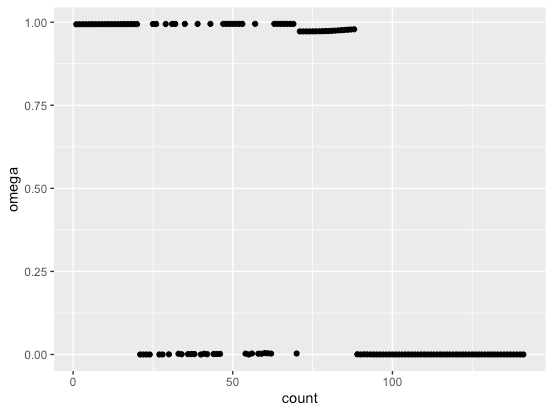
\includegraphics[width=0.35\textwidth]{img/Spring_2022_Journal-b16835c7.png}
	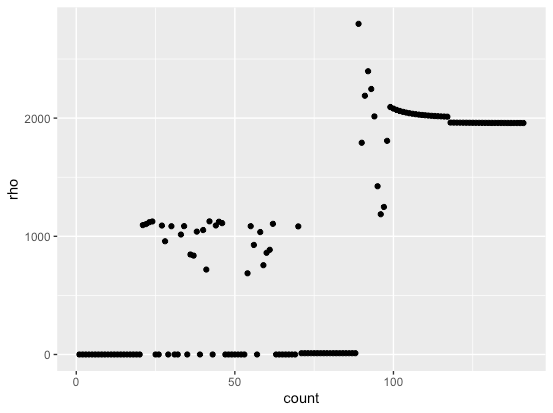
\includegraphics[width=0.35\textwidth]{img/Spring_2022_Journal-504ae687.png}


With this last run, the last betas seem to be reasonable numbers, between -10 and 10 and roughly normally distributed, although a couple around -40 and -30

Did work on data best practices: Save all test datasets so dont have to rerun code. Currently have 10, 20 and 30 percent filtering, with the one covariate.


\subsection{Filtering of 20 percent}

With rho start value of 10. Difference is 0 after 2 iterations.
What if stronger tolerance? try diff > .01


Should save convergence results of nls optim.

Quickly add new covariate on med dataset. Then go to line search. Hopefully will help with stability?

Still high value of omega, rho 11.

Somewhat normally distributed betas, with some very large ones, same for residuals.

Try the "larger" dataset with minus:
Stop after first iteration: Infinite values due to infinite valued alpha or A.

Seems to be really popping back between omega as 0 and 1 and rho as .05 and 1000.

Back to using 30 percent
Also note that gamma is at .05

When gamma is .05 and rho is 10, ends in 3 iterations...

When gamma is .1, rho 10, still get omega .9, rho small

Original omega .8, rho 4

Tried back to gamma of .05 and it works...

\end{document}
